% !Mode:: "TeX:UTF-8"

\BiChapter{密集热点区域无线网络的优化}{UDN optimization}

根据第三章的分析,在不采用任何干扰管理和协调算法的情况下,网络中能达到正常工作的信干噪比的用户占总共的用户量的百分比很低。
从而导致了反应网络中所有用户有效性的平均的性能的单位面积谱效率也很低。
因此需要设计一种干扰管理和协调算法提升网络的性能。

本章从两个角度进行分析,即将分两步进行干扰管理和协调,第一步对小区中的微基站进行分簇,从而达到边缘用户减少,
第二步对每个簇中的基站采用~CRAN~网络架构进行联合,由于~CRAN~架构可以将不同微基站的基带信号传输至云化的~BBU~池进行统筹处理。
在~BBU~池侧,可以采用联合传输预编码的方法将发送给不同用户的信息在空域上相互正交,从而达到干扰消除的目的。
\BiSection{密集热点区域无线网络的干扰管理算法的架构}{algorithm construction}
根据图~\ref{e_capacity_show}~显示的结果,在小区中心的用户,收到的干扰较小,遍历容量较好,能达到正常通信的遍历容量需求。
小区边缘的用户的遍历容量较差,反应了小区边缘收到的干扰较为强烈,
接收信干噪比较低,处于边缘的终端出现中断的概率很大,因此要想办法去让边缘用户的性能提升,从而降低网络的中断概率,提高网络覆盖率。

联合传输技术是伴随第四代移动通信~(4G)~提出的一个关键技术。其主要的思想是以用户为中心,将基站联合起来,进行协作,共同对用户进行服务。
由于基站间相互联合共同服务区域内的用户用户,
处在基站边缘的用户的干扰功率也能被用户利用成为有用的接收功率,从而使得边缘用户的有效性大大提升。
联合传输中,网络由用于处理数字信号的BBU池,用户传输信号的微基站和前向回程链路组成。
传送给用户的信息首先通过BBU池进行数据处理,在通过前向回程链路传输到基站端,由于采用了干扰消除算法,因此两个基站传送给用户的信息均为用户可以利用的有效信号,
实现两个基站联合传输共同服务区域内的用户的目的。

在第三章中,定义了网络的网络中基站的拓扑结构,用户的统计特性,信道的基本模型。
即在面积为~$\mathcal{A}$~的区域中,基站的分布~$\Phi$~是一次泊松点过程的实现,
其密度参数为~$\lambda_s$,基站的个数为~n~个,用户在网络中的分布在微基站附近的分布更多,
随着距离基站越来越远,用户出现的概率越小。
假设用户服从以基站位置为均值的混合二维高斯分布,定义物理量~$\sigma$~表示用户的发散程度,量纲为米。
其中~$\sigma$~表示混合二维高斯分布的标准差。
在之前的分析中,由于没有采用多用户联合传输技术,因此所有基站的功率假设是等功率的,
而采用了联合传输以后,可以对所有的基站进行统一的调度,因此网络可以进一步通过功率控制的方法进行优化。
现假设基站~$S_i$~的最大发射功率为~$P$。
除此之外,本文采用的多用户联合传输中,为了进行干扰管理,采用预编码的技术进行干扰消除,预编码矩阵为~$\mathbf{W}$。
用户~$U_j$~接收到基站~$S_i$~的接收功率受到基站~$S_i$~的最大的发射功率~$P$,预编码矩阵~$\mathbf{W}$,描述信道的大尺度衰落的信道衰减系数~$\alpha$,
描述瑞利信道的随机变量~$h$决定。

 假设采用~BPSK~调制方式,在小区中一共有~$k$~个用户~$n$~个基站,
 基站发射给用户的信息为~$\mathbf{q}=\{q_1,q_2,\dots,q_j,\dots,q_k\}$,
 其中~$q_j\in\{1,-1\}$~表示用户~$U_j$~想要接收到的信号。
 在进行预编码之前需要首先要确定每个用户所需要分配的功率。
 在进行功率分配后,待发射的信号~$\mathbf{x} = \{x_1,x_2,\dots,x_j,\dots,x_k\} = \{p_1 q_1,p_2 q_2,\dots,p_j q_j,\dots,p_k q_k\}$。
 其中为~$\mathbf{p}=\{p_1,p_2,\dots,p_j,\dots,p_k\}$~为功率分配权重。
 因此用户~$j$~分配到的功率的值为~${p_j}^2$~

 预编码矩阵为~${\mathbf{W}=\{w_{ij}\}}_{n\times k}$。
 其中~$w_{ij}$~表示第~$j$~个用户所发送的信息在第~$i$~个基站所占的权值。则基站的发射信号向量~$\mathbf{s}$可表示为:
 \begin{equation}\label{send_s}
   \mathbf{s}=\mathbf{W} \mathbf{x}
 \end{equation}
其中~$\mathbf{x}$~为发射信号的向量,$\mathbf{W}$~为预编码矩阵,
可将预编码矩阵~$\mathbf{W}$~表示为~$n\times 1$~的分块矩阵
~$\mathbf{W}=\{\mathbf{w}_1, \mathbf{w}_2,\cdots,\mathbf{w}_k\}^{\mathrm{T}}$。
在联合传输的过程中,所有的基站共享用户的发送信息和信道状态信息,
以得到状态信息作为参数,得到的预编码矩阵,即可以对网络的有效性进行优化,
通过预编码矩阵修改发送每个用户信息的权重,
将加权后的信号交由基站进行发送。

基站发送的信号受到大尺度衰落和小尺度衰落的影响。
定义系数矩阵~$\mathbf{G}=\{g_{ij}\}_{k\times n}$,
其中~$g_{ij}\in\mathbb{R}$,$g_{ij} = h_{ij}R_{ij}^{-\alpha}$,
其中~$h_{ij}$~和~$R_{ij}$~分别表示基站~$S_i$~和用户~$U_j$~之间的信道系数和距离。
用户的接收信号向量~$\mathbf{y}$~为:
\begin{equation}\label{received_y}
  \mathbf{y} = \mathbf{Gs} + \mathbf{z}
\end{equation}
其中~$\mathbf{G}$~为信道的系数矩阵,$z\in \mathbb{R}$~为加性高斯白噪声,噪声的功率谱密度为~$N_0$。

若采用基于~ZFBF~的多用户联合传输技术,则预编码矩阵~$\mathbf{W}$~为:
\begin{equation}\label{precode_w}
  \mathbf{W} = \mathbf{G}^{\mathrm{T}}(\mathbf{G}\mathbf{G}^{\mathrm{T}})^{-1}
\end{equation}
其中~$\mathrm{T}$~表示转置,即采用基于~ZFBF~的多用户联合传输技术的情况下,
预编码矩阵为信道系数矩阵的广义逆。

将式~(\ref{send_s})~和式~(\ref{precode_w})~带入到式~(\ref{received_y})~中,
可以得到接收信号关于发送信号~$\mathbf{x}$~和噪声~$\mathbf{z}$~的表达式:
\begin{equation}
  \mathbf{y} = \mathbf{x} + \mathbf{z}
\end{equation}

由于干扰通过基于~ZFBF~的多用户联合传输技术已将消除掉了,
因此用户的接收信干噪比与信噪比相同,用户~$j$~的信干噪比~$\gamma_{j}$~如式~(\ref{gamma_r})~所示:
\begin{equation}\label{gamma_r}
  \gamma_j = \frac{{x_j}^2}{N_0}= \frac{{p_j}^2}{N_0}
\end{equation}
用户~$U_j$~的容量的表达式为:
\begin{equation}
  R_j = \log_2(1+\gamma_j)
\end{equation}

可以看到簇内干扰被消除掉,容量只受接收到的有用功率和噪声的影响。
联合传输可以统筹信道状态信息,用户的发送信息,可以采用多基站写作的方法对干扰进行抑制,
达到提升网络性能的目的。
不仅如此,由于基站可以通过一个中心控制器进行统一的调度,可以选取不同的目标函数,
使网络的某些特定性能,如覆盖率,单位面积频谱效率达到最优,实现网络优化的目的。

虽然联合传输可以技术可以提升边缘用户的通信性能,提高覆盖率,
提升网络的和速率,最大化单位面积频谱效率,
但是联合传输技术并不能直接用于密集热点区域无线网络当中,在密集热点区域无线网络中,
区域内的基站较为密集,基站的分布是不均匀的,
且一般情况下数量较多,如果将区域内的所有基站全部都联合在一起,系统的复杂度很高,实现难度太大。

为改进联合传输技术,使其不但能增加使处在服务区域边缘的用户的传输可靠性,提升网络的性能,又能有较低的复杂度。
本文提出的干扰管理算法分为两个步骤,首先,对小区中的微基站进行分簇,将簇内的基站整体作为协作集,共享信道的发送信息与信道状态信息。
然后再对每个簇中的基站采用~CRAN~网络架构进行联合,对同一个簇中的用户采用联合传输策略,
将簇内发送给各个用户的有用信号在空域上尽可能的正交,
增强发送给用户的有用信号,
抑制用户接收到的干扰,
达到增加网络的覆盖率,提升网络的区域面积频谱效率的目的。
网络的示意图如图~\ref{CoMP_cluster}~所示:
在图中,将小区内的~5~个基站分成了三个簇,分别为簇~A,簇~B和簇~C,当簇内含有多个基站时多用户联合传输的网络架构,
通过云服务器对发送的信号进行集中的数字信号处理。
对簇内采用干扰管理和协调算法,但不同簇的基站之间会产生簇间干扰。

\BiSection{密集热点区域无线网络的基站分簇}{clustering of basestation in UDN}

本小节对密集热点区域无线网络的基站的分簇算法进行研究,提出基于深度优先搜索的网络中微基站分簇算法。
将距离相聚过近的基站进行联合,
消除由基站过近导致的强烈的干扰,
也避免由于基站之间相距过近而导致边缘用户较多的情况发生。

本节将深度优先搜索算法和~k~-~均值算法应用到网络的分簇当中。下面分别介绍基于上述两种算法的网络分簇方法。
\begin{figure}[htbp]
\centering
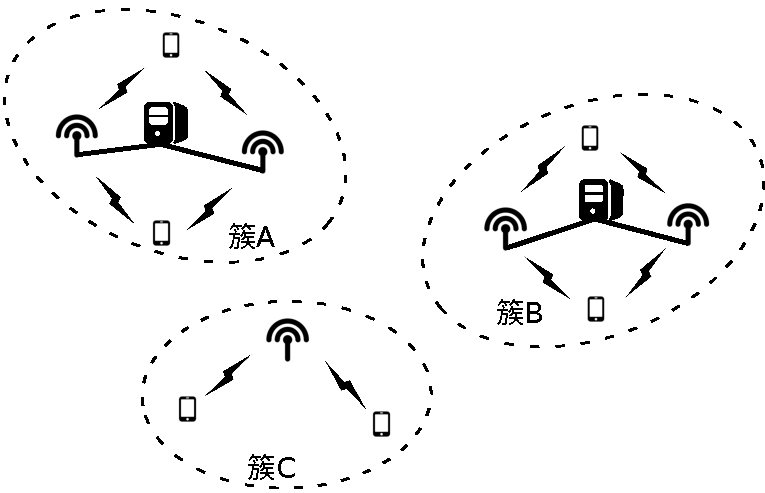
\includegraphics[width = 0.7\textwidth]{CoMP_cluster.pdf}
\caption{密集热点区域无线网络的干扰管理架构示意图}\vspace{-0.5em}
\label{CoMP_cluster}
\end{figure}
\BiSubsection{基于深度优先搜索的微基站分簇算法}{Time diversity}
根据图~\ref{e_capacity_show}~所示,相邻的基站之间如果距离过近,则由于基站之间的干扰强烈,小区中用户的遍历容量性能,
网络的覆盖率和单位面积频谱效率性能将会受到巨大的影响,除此之外,如果两个基站的距离过近,
由于微基站服务的区域用户量需求大,
容量要求高,因此两个基站之间会存在大量的边缘用户,从而极大的影响了系统的性能。

为了避免基站相聚过近而导致的基站之间的干扰强烈,边缘用户过多。
本小节提出了基于深度优先搜索的基站分簇算法。
深度优先搜索算法是计算机科学当中的基础算法,也是图论当中比较经典的算法之一。

下面介绍基于图的深度优先搜索的为基站分簇算法,为了应用按深度优先的搜索,首先需要在将网络中的基站拓扑映射成为一个图结构。
给定区域~$\mathcal{D}$~中的所有基站
~$\mathcal{S}(x,y)=\{S_1(x_1,y_1), S_2(x_2,y_2),\dots,S_i(x_i,y_i)~,\dots,S_n(x_n,y_n)\}$,
其中~$x$,$y$~分别表示基站的横,纵坐标。
对任意的~$i,j\in\{1,2,\dots,n\}$,基站~$S_i$~与基站~$S_j$~之间的距离为~$R_{ij}$,
根据微基站集合~$\mathcal{S}$~和基站之间的距离~$R_{ij}$,$i,j \in\{1,2,\dots,n\}$构造图~$\mathcal{G}$,
其中图~$\mathcal{G}$~的节点集合~$\mathcal{V}=\{v_1,v_2,\dots,v_i,\dots v_n\}$~
为微基站集合~$\mathcal{S}$~的一一映射,即对任意给定的~$i\in\{1,2,\dots,n\}$,
存在映射关系~$S_i \rightarrow v_i$。图~$\mathcal{G}$~的所有边构成的集合~$\mathcal{E}$~
根据微基站之间的距离是否小于门限~$\tau$~决定,即对任意的~$i,j\in\{1,2,\dots,n\}$,若~$R_{ij}<\tau$,
则存在边~$e_{ij}\in\mathcal{E}$,
表示图~$\mathcal{G}$~中存在边~$e_{ij}$~将节点~$v_i$~和节点~$v_j$~连接。
根据图~$\mathcal{G}$~的边集合~$\mathcal{E}$,可以构造邻接矩阵~$\mathbf{A}=\{a_{ij}\}_{n\times n}$,其中
\begin{equation}
a_{ij}=
\begin{cases}
1, & e_{ij}\in \mathcal{E}, \\
0, & e_{ij}\notin \mathcal{E}.
\end{cases}
\end{equation}

在~$\mathcal{G}$~中,定义两个节点~$v_i$~和~$v_j$~是连通的,则从定点~$i$~到定点~$j$~有路径相连。
基于深度优先搜索的基站分簇算法将所有连通的节点划归为一簇,
将图~$\mathcal{G}$~划归为由不同子图构成的不交并,
由于图上的节点和微基站之间有一一映射的关系,
属于同一个子图的节点相互连通。
可将处在同一个子图上的节点对应的基站划分成为一个簇。
即~$\mathcal{S} = \dot{\bigcup\nolimits}_{i=1}^{m}\mathcal{C}_i$,
表示将基站的集合~$S$~分成了~$m$~个子集合,每个集合里的基站构成一簇。
完整的描述如算法~\ref{algorithm_bs_dfs}~所示:


\begin{algorithm}[!htb]
\caption{ 基于深度优先搜索的基站分簇算法 }
\label{algorithm_bs_dfs}
\small
\SetKwProg{Fn}{Function}{}{end}
\KwIn{  $\tau$~;$\mathcal{S}(x,y)$}
\KwOut{ $\mathcal{K}$ }
\Begin
{
    第~1~步:初始化\\
    $\mathbf{A}=\{a_{ij}\}_{n\times n}=\{0\}_{n\times n}$~;
    $c=0$~;
    $\mathcal{K}=\varnothing$~;
    $\mathbf{v}=\{v_i\}_n=\{0\}_n$~\\

    第~2~步:构造邻接矩阵~$\mathbf{A}$:\\
    \For{~$i=1 \ to \ n$,$j=1 ~ to ~ n$~}
    {
          $a_{ij}=(\sqrt{({x_i} - {x_j})^2+(y_i-y_j)^2} < 0~)$  \\
    }
    第~3~步:构造深度优先搜索函数:\\
    \Fn{$DFS$(~$node$~$i$~, $\mathcal{C}_c$~)}
    {
      \For{~$j=1\ to\ n, j \neq i$~}
      {
        \If{~$v_j==0 \ \ and\ \ a_{ij} == 1$~}
        {
          $v_{j}=1$ \\
          $\mathcal{C}_c=\mathcal{C}_c \bigcup~ \{~S_j~\}$\\
          $\emph{DFS(~j~,~}\mathcal{C}_c ~\emph{)}$\\
        }
      }
    }
    第~4~步: 基于深度优先搜索的基站分簇\\
    \For{~$i=1 \ to \ n$~}
    {
      \If{~$v_i == 0$~}{
        $c ~+= 1$ \\
        $\mathcal{C}_c = \{~S_i~\}$\\
        $v_i = 1$\\
        $\emph{DFS(~i~,~}\mathcal{C}_c ~\emph{)}$\\
        $\mathcal{K} = \mathcal{K} \bigcup~ \{~\mathcal{C}_c~\}$\\
      }
    }
}
\end{algorithm}

算法的输入为距离门限~$\tau$和基站的坐标参数~$\mathcal{S}(x,y)$,
算法分为四个步骤执行。

其中第一步为初始化步骤,
将邻接矩阵~$\mathbf{A}$~初始化为~$\mathbf{0}_{n\times n}$,
将网络中微基站簇的个数~$c$~设置为0个,
微基站簇的集合~$\mathcal{K}$~设置为空集~$\varnothing$,
用于标识是否与微基站一一映射的节点是否访问过的向量~$\mathbf{v}$~设置为~$\mathbf{0}_{n\times 1}$,
对应位置为~0~表示未被访问,为~1~表示已经被访问。

算法的第二步为构造邻接矩阵,
对任意的基站~$S_i$~和~$S_j, ~i, ~j \in \{~1,~2,\cdots,~n~\}$,
当基站之间的距离小于门限~$\tau$,则邻接矩阵对应的位置~$a_{ij}=a_{ji}=1$,
否则邻接矩阵对应的位置~$a_{ij}=a_{ji}=0$。

算法的第三步为构造邻接矩阵的深度优先搜索的矩阵,
深度优先搜索用于将与给定的节点~$i$~的所有连通的节点全部搜索出来,构成集合~$\mathcal{C}$~。
首先将节点~$i$~对应的基站~$S_i$~放入集合~$\mathcal{C}$~中,
并将向量~$\mathbf{v}$~中的第~$i$~位~$v_i$~置~1,
接着采用递归的方法依次遍历所有除给定节点~$i$~以外的节点,
如果存在节点~$j$~与给定节点~$i$~相连通且未被遍历,
则将微基站~$S_j$~放入集合~$\mathcal{C}$~中,
并将向量~$\mathbf{v}$~中的第~$j$~位~$v_j$~置~1,
从节点~$j$~开始继续执行按深度搜索的遍历,
直到所有与给定节点~$i$~连通的节点都被找到为止。
通过深度优先搜索函数可以得到网络中的一簇基站。

算法的第四步应用第三步给出的深度优先搜索函数,从~1~到~$n$~依次开始遍历整张图,
如果节点~$i$~未被分簇,通过函数找到与节点~$i$~连通的所有节点作为一簇。
直到所有的节点均被分簇为止。


算法通过给定距离门限,将小于距离门限的所有基站连接在了一起。这些基站共同给所覆盖区域内的用户进行服务。
从而极大的降低了边缘用户的数量,增大了用户所接收到的有用功率,减小了用户接收到的干扰。

但是,由于小区中基站的部署是泊松点过程,因此,小区中的基站的分布并不均匀,
因此可能会出现某个协作集当中的基站过多,
从而可能导致多用户簇内的多用户联合传输的复杂度过高。
不仅如此,由于小区中的微基站采用了以基站为中心的分簇方式。
小区中的服务范围依然存在明显的边界,处在边界上的用户依然会可能会受到比较严重的干扰。

\BiSubsection{基于~k~-~均值的微基站分簇算法}{Time diversity}
K~-~均值算法是人工智能领域常用的一种非监督学习算法\citeup{InfoTheoryInference}。
其是一种基于迭代的统计学习方法,由~Dempster~等人总结提出,
是均方最大(~EM~)算法的一种特例\citeup{statisticslearning}。
算法的主要步骤分为两步,即分配步骤和更新步骤。
功能分别为设定权重矩阵和更新均值点集。
与机器的思考方式不同,人类可以很容易的辨识区域内的物体,并将这些物体分类。
但若要让计算机也可以对空间内的点集进行分簇,
需要采用聚类算法,将簇内基站相距距离较近,并且与簇外基站相距较远,
并且由于算法存在均值,一个簇所划归的区域近似为一个圆形。
k~-~均值算法首先随机生成~k~个点作为均值的初始点,均值点的集合用~$\mathcal{M}$~表示,
$\mathcal{M}=\{~M_1(x_1,y_1),~M_2(x_2,y_2),\dots,~M_k(x_k,y_k)~\}$。
将每个均值附近的点作为一簇,再通过簇内点集迭代出新的均值。
直到算法收敛或迭代次数耗尽为止。

在密集热点区域无线网络覆盖的区域~$\mathcal{D}$~上,
已知微基站的位置坐标集合~$\mathcal{S}(x,y) = \{S_1(x_1,y_1), S_2(x_2,y_2),\dots,S_n(x_n,y_n)\}$。
用~k~-均值算法将点集~$\mathcal{S}(x,y)$~分成~K~个簇~$\mathcal{S} = \dot{\bigcup}_{i=1}^{k} \mathcal{C}_i$。
对任意的~$i\in\{~1,~,2,\dots,~n~\}$,$j\in\{~1,~2,\dots,~k~\}$,
$d(~S_i,~M_j~)$~表示微基站~$S_i$~和均值~$M_j$~之间的距离。算法的描述如算法~\ref{kmeansalgorithm}~所示:
\begin{algorithm}[!htb]
\caption{ 基于~k~-均值聚类的基站分簇算法 }
\label{kmeansalgorithm}
\small
\SetKwProg{Fn}{Function}{}{end}
\KwIn{$k$~;$\mathcal{S}(~x,~y~)$~;$iter$}
\KwOut{$\mathcal{M}$}
\Begin
{
    第1步:初始化\\
    随机生成~k~个坐标~$\mathcal{M}=\{~M_1,~M_2,\cdots,~M_k~\}$~构成均值点集;\\
    生成权值矩阵~$\mathbf{C}=\{~0~\}_{n\times k}$~;\\
    迭代次数~$count=0$~\\

    第2步:~k~-~均值算法:\\
    \While{~$count++ < ~iter$~}
    {
      步骤~2.1:设定权重矩阵\\
      $\mathbf{C}=\{~c_{ij}~\}_{n\times k}=\{~0~\}_{n\times k}$\\
      \For{~$i=1 \ to \ n$~}
      {
        $\hat{j}=\arg\min\limits_{j} ~d(~S_i,~M_j~)$ \\
        $c_{i\hat{j}}=1$  \\
      }

      步骤~2.2~:均值点集更新:\\
      \For{~$j=1 \ to \ k$~}
      {
        $C_j = \sum_{i=1}^n c_{ij}$  \\
        $M_j(~x_j, y_j~) = \frac{\sum_{i=1}^{n} c_{ij} S_i(~x_i,~y_i~)}{C_j}$  \\
      }
    }
}
\end{algorithm}

首先输入基站分簇的簇的个数~k~,微基站的坐标~$\mathcal{S}(~x,y~)$,迭代次数~$iter$。
算法主要分为两步,第~1~步为初始化部分,随机生成~k~个点作为均值点的初值,
权重矩阵~$\mathbf{C}$~设定为全~0~矩阵,设定迭代次数~$count$~为~0。
算法的第~2~步为~k~-~均值算法的实现,是一个迭代的过程,迭代的次数为~$iter$~次。
迭代的过程分为两个子步骤,子步骤~2.1~找遍历所有的微基站,找到距离微基站最近的均值点,
将权重矩阵~$\mathbf{C}$~相应的位置置~1。
子步骤~2.2~用得到的权值矩阵~$\mathbf{W}$~
对基站的坐标~$\mathcal{S}(~x,~y~)$~进行权值更新得到新的均值集合~$\mathcal{M}$。

基于~k~-均值算法的聚类可以对基站进行分簇,与基于深度搜索算法的基站分簇不同,
基于~k~-~均值算法的基站分簇将区域内的基站均匀的分配到~k~个簇当中,
每个区域的大小也近似相同,是一种有效的基站分簇算法。
并且基于~k~-~均值的基站分簇算法可以的到网络的中心,
簇的大致位置可以通过均值的信息反映出来。

基于~k~-~均值算法的基站分簇需要预先设置好簇的个数,
为了得到最优的簇的个数,
需要进行多次试验。
不仅如此,算法需要通过迭代实现分簇,算法的复杂度较高。
由于算法并不是依据基站之间的关系进行分簇,因此也没有利用基站之间的拓扑结构这一信息。

\BiSubsection{以用户为中心的基站分簇算法}{Time diversity}

根据前面的讨论,我们提出了在密集热点区域的场景下的基站分簇算法,
分簇算法都是以基站为中心的,其中,
基于深度优先搜索的基站分簇算法将距离近的基站选择在一起作为协作基站,
达到解决边缘用户过多,网络系统的覆盖率性能过差的网络中所面临的问题,
但算法虽然对网络的覆盖率的性能取得了提升,由于簇内干扰的到了消除,
簇内的基站之间的边缘用户的性能大大的提升了,
但是由于簇间的干扰不能通过之前提出的算法进行消除,因此处在簇间边缘的用户依然会受到较强的干扰,
不利于系统覆盖率性能的进一步提升。
除此之外,由于网络模型是随机的,因此会存在有的区域内,基站稠密,有的区域基站稀疏,
导致分簇的结果是不均匀的,有的簇的簇内基站多,有的簇的簇内基站少,如果簇内的基站过多,
系统将面临复杂度过高的困扰。
基于~k~-~均值的基站分簇算法,通过机器学习中的~k~-~均值算法,将基站较为均匀的进行分簇,
但是距离过近的基站可能会处在不同簇中,簇间边缘的用户数量没有得到控制。

上述问题在以基站为中心的网络中是难以解决的,但如果已知用户的位置,可以对分簇算法进行进一步的优化。
用户的位置信息已知,则可以将用户的接收信干噪比估算出来,通过用户的接收信干噪比要求,
以用户为中心设定距离门限,将以用户为中心,以距离门限~$\tau$~为半径内的基站选为协作基站,
以提升网络的性能。

在区域~$\mathcal{D}$~中,基站的分布服从泊松点过程~$\Phi$,基站的密度为~$\lambda_s$,基站的个数为~$n$,
用户的分布~$\Psi$~为以基站为均值的混合二维高斯分布。
以用户为中心的基站分簇算法需要给定用户的位置信息
~$\mathcal{U}(~x,~ y~)=\{~U_1(~x,~y~),~U_2(~x,~y~),\dots,~U_k(~x,~y~)~\}$,
不失一般性的假设每个基站所处的热点的热度相同,每个基站的热点影响且只影响一个用户,
用户随机生成,每个用户的坐标为以影响他的热点基站的坐标为均值,
用户的分散程度的平方为方差的二维高斯分布的随机数。

在上一章对当网络未采用协作的情况下的覆盖率做出了讨论,本章将对上一章的结果做进一步的展开,
由于用户~$i$~的位置是已知的,因此可以讨论用户处在固定位置~$O$~上,
已知距离其最近的基站的距离~$r$,当距其最近的干扰基站的距离为~$R$~时,
用户的信干比性能~$\gamma_r$~大于~$T$~的概率~$\mathbf{P}(~\gamma_i > \Gamma~)$。

当有用信号的信道系数未知的情况,对公式~(\ref{Ls})~做变型,
即可得到~$\mathbf{P}(~\gamma_i > T \mid r,R~)$,如式~(\ref{p_r_R})~所示:

\begin{equation}\label{p_r_R}
  \mathbf{P}(~\gamma_i > T \mid r,R~)
  {=}  \exp\left(-2\pi\lambda_s\int_{R}^{\infty}
          \left(1 - \frac{1}{1+ T r ^\alpha v^{-\alpha}}\right)\mathrm{d}v\right)
\end{equation}
%该种情况适合信道状态信息变化较快的情况。
给定信干噪比~$\gamma_i$~要求,
给定终端概率~$\mathbf{P}(~\gamma_i < T \mid r,~R~)$~要求,
给定距最近基站的距离,即可得到需要保证非簇内的基站与用户的最近的距离,
从而根据得到的结果设定距离门限~$\tau$。

定义~$\rho(T, \alpha)$~如式~(\ref{rho})~所示,对等式变形,可得:
\begin{equation}
  \mathbf{P}(~\gamma_i < T \mid r,~R~) = \exp\left[-\pi R^2 \lambda_s~ \rho\left((r/R)^\alpha T, \alpha\right)\right]
\end{equation}




%当用户的有用信号的信道状态信息已知的情况下,
%可以对中断概率做更准确的分析,从而得到更精确的距离门限~$\tau$。
%下面对中断概率做进一步的分析,
%根据用于服务用户的微基站~$S_0$~发射的有用信号的的发射功率~$P$,信道系数~$h$~和距最近基站的距离~$r$,有用接收功率的表示为:
%\begin{equation}
%  P_r= h r^{-\alpha} P
%\end{equation}
%因为信道状态信息已知,在不采用其他的处理手段的情况下,用户的接收功率是已知的。
%干扰基站~$S_i$~与用户之间的距离为~$R_i$,信道为瑞利分布,信道系数~$h_i$~服从单位指数分布~$h_i\sim\exp~(1)$。
%干扰基站对用户的总的干扰功率的表达式为:
%\begin{equation}
%  I_r = \sum_{S_i \in \Phi \backslash S_0} h_i R_i^{-\alpha} P
%\end{equation}



\BiSection{密集热点区域无线网络的簇内干扰消除与优化}{algorithm construction}

\BiSubsection{CRAN~架构下基于分布式预编码的簇内干扰管理}{Time diversity}
为消除密集热点区域无线网络的簇内干扰,提出基于分布式迫零预编码的干扰消除技术。
其中发射端采用~CRAN~架构,即将所有基站的基带处理单元集中在一起,构成基带处理单元池(~BBUs~),
在基站端退化为远端射频头(~RRHs~),进行模数转换与射频收发功能,并将用户的信道状态信息
传送到~BBUs,实现基于信道状态信息的迫零预编码。
簇内干扰消除的原理框图如图~\ref{precode_inner_cluster_show}~所示:
\begin{figure}[htbp]
\centering
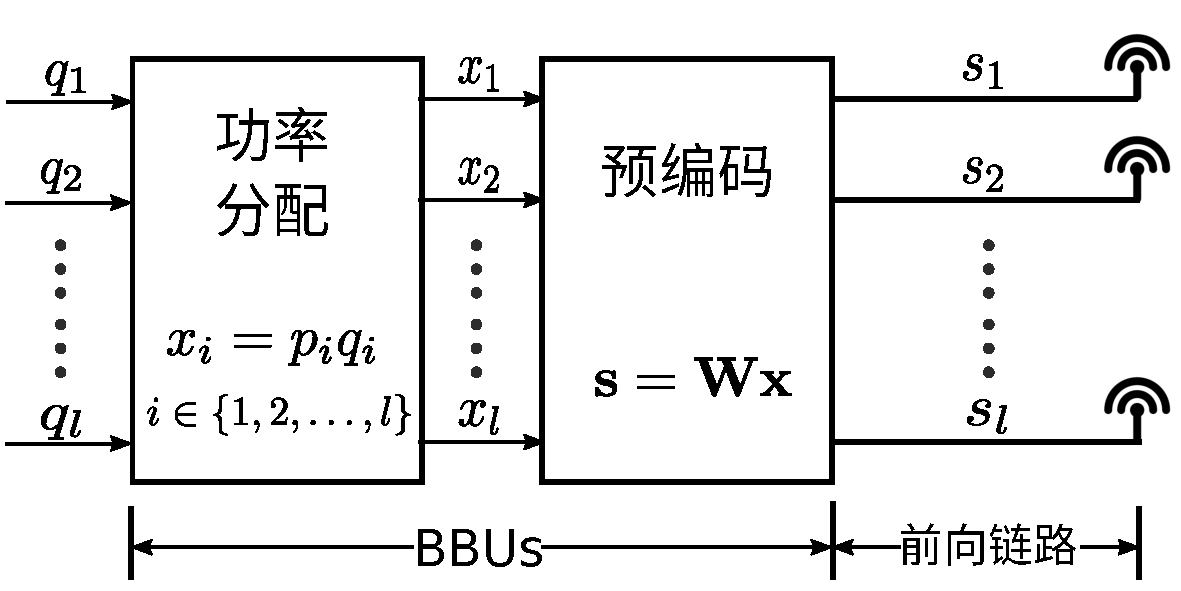
\includegraphics[width = 0.85\textwidth]{precode_inner_cluster_show.pdf}
\caption{CRAN~架构下基于分布式预编码的簇内干扰管理架构图}\vspace{-0.5em}
\label{precode_inner_cluster_show}
\end{figure}
假设在一个簇内存在~$l$~个基站,在每个基站所覆盖的区域内随机选择一个用户即一个簇内
同时对~$l$~个用户进行服务。
在~BBUs~中对基带信号进行处理,待发射的信号向量为~$\mathbf{q}=\{~q_1,~q_2,\dots,~q_l~\}, ~q\in\{~\pm 1~\}$。
在基于迫零预编码的簇内干扰管理算法中,首先要给待传送的信号进行功率分配。
每个用户所分配的功率由功率分配因子~$\mathbf{p}$~决定。
功率分配过后的信号~$\mathbf{x}=\{~p_1q_1,~p_2q_2,~\dots,~p_nq_n~\}$。
对经过功率分配后的信号向量进行迫零预编码,得到待发送的信号~$\mathbf{s}=\mathbf{W}x$。
其中迫零预编码的预编码矩阵
~$\mathbf{W}=\mathbf{G}^{\mathrm{T}}(\mathbf{G}\mathbf{G}^{\mathrm{T}})^{-1}$。
其中~$\mathbf{G}=\{g_{ij}\}_{~l~\times~ l}=R_{ij}^{-\alpha}h_{ij}$。其中~$R_{ij}$~
为基站~$S_i$~和用户~$U_j$~之间的距离,$h_{ij}$~为瑞利信道下基站~$S_i$~和用户~$U_j$~
的信道系数。
得到了经过预编码矩阵得到的待发送信号~$\mathbf{s}=\{~s_1,~s_2,\dots,~s_l~\}$,基带信号的处理完成,
对任意的~$i\in\{~1,~2,\dots,~l~\}$,$s_i$~表示需要微基站~$S_i$~去发送的信息。
将发送信号~$\mathbf{s}$~通过前向回程链路传送给微基站~$\mathcal{S}$,
此时不同用户的信息彼此之间相互正交,因此不会受到来由于使用同时同频资源而造成的用户之间的干扰。

\BiSubsection{簇内用户的功率资源分配}{Time diversity}
根据上一小节的内容,在进行预编码之前,首先需要进行功率分配。
本小节提出等功率分配方式,分别为等功率分配和最大化基站功率使用的功率分配。
其中,等功率分配假设每个微基站的天线上所能承载的最大的功率已知,系统基于公平性的原则,
希望每个用户分配到相同的功率。
最大化功率使用的功率分配方法不需要每个用户分配到的功率均是相等的,
而是希望尽可能的使用基站的功率,从而使得所有的用户分配到的总的功率最大化。

等功率分配需要满足每个用户分配的功率是相等的。但经过预编码后信号需要满足功率约束条件。
预编码矩阵~$\mathbf{W}$~可以写成分块列向量的形式
~$\mathbf{W}=\{~\mathbf{w}_1,~\mathbf{w}_2,\dots,\mathbf{w}_l~\}$,
假设微基站所能提供的最大功率为~$P$~则功率约束条件为:
\begin{equation}\label{P_constrain}
  {s_i}^2 = (\mathbf{w}_i \mathbf{x})^2 = \sum_{j=1}^l (w_{ij} p_j q_j)^2
  = \sum_{j=1}^l (w_{ij} p_j)^2 \leq P ,~ i\in \{~1,~2, \dots, ~l~\}
\end{equation}
由于采用等功率分配,~$p_1=p_2=\cdots=p_l=p$~上式可以变形为:
\begin{equation}
  \sum_{j=1}^{l} (w_{ij}p)^2 \le P ,~ i\in \{~1,~2, \dots, ~l~\}
\end{equation}
根据功率分配约束,可以得到功率分配因子:
\begin{equation}
  p=\frac{1}{\min\{~\sum_{j=1}^{l} (w_{1j})^2,~\sum_{j=1}^{l} (w_{2j})^2,\dots,~\sum_{j=1}^{l} (w_{lj})^2~\}}
\end{equation}
由于在超密集组网场景中,网络为一个干扰受限的网络,因此对网络起主要影响的是基站之间的干扰。
而对簇内采用了迫零预编码技术,簇内用户的信息在不同的向量空间当中。
簇内的干扰完全的得到了消除,是否使得簇内和速率达到最优与否其性能的影响可以忽略不计。

\BiSection{密集热点区域无线网络优化的性能分析}{analysis}
\BiSubsection{网络分簇算法的分析}{cluster}

在第三章,我们给出了网络仿真的网络示意图~\ref{network_dis_show},
对基于深度优先搜索算法的基站分簇算法得到的分簇结果进行仿真,
仿真参数如表~\ref{dfs_show_sim_para}~所示:
\begin{table}[htbp]
\caption{基于深度优先搜索的分簇算法的仿真参数}
\label{dfs_show_sim_para}
\vspace{0.5em}\centering\wuhao
\begin{tabular}{cccc}
\toprule[1.5pt]
参量 & & & 设置 \\
\midrule[0.5pt]
基站的分布~$\Phi$~ & & & 泊松点过程 \\
泊松点过程的密度参数~$\lambda_s$~ & & & ~$0.01~\mathrm{m}^{-2}$~ \\
区域的大小  & & & ~$100\mathrm{m} \times 100 \mathrm{m}$~ \\
基站的个数~$n$~  & & & 100\\
深度搜索的距离门限~$\tau$~ & & & ~$5\mathrm{m}$~\\
\bottomrule[1.5pt]
\end{tabular}
\end{table}

选取的区域的大小为 ~$100\mathrm{m} \times 100 \mathrm{m}$~的正方形的区域,
正方形的区域中的基站的部署为泊松点过程,密度参数为~$\lambda_s=0.01 \mathrm{m}^{-2}$,
距离门限~$\tau=5~\mathrm{m}$。
对生成的这片区域采用基于深度优先搜索的分簇算法,得到的网络示意图如图~\ref{dfs_network_show}~所示:
\begin{figure}[htbp]
\centering
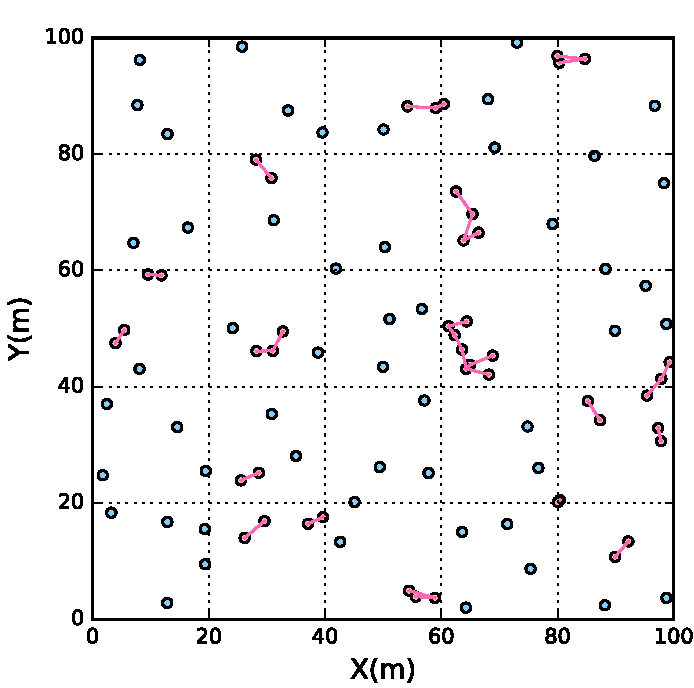
\includegraphics[width = 0.5\textwidth]{dfs_network_show.pdf}
\caption{基于深度优先搜索的分簇算法的效果图}\vspace{-0.5em}
\label{dfs_network_show}
\end{figure}
其中的蓝色的点表示独立的微基站,粉色的点表示使用了多用户联合传输的微基站。
如果微基站的节点之间有一条边相连,则两个基站同属于一个簇。
可以看到,当两个基站的距离~$R_{i,j} < 5$~时,基站就会被连接在一起,共同的归于一个簇。
验证了算法的正确性。
由于密集热点区域的用户具有集中性,因此当两个基站之间的距离过远时,处在边缘的用户更少。
除此之外,基站之间的距离较远,所服务的用户距离干扰基站的距离更远,有效的避免了基站相聚过近的干扰,以及处在边缘的用户的数量过多对性能的影响。

对基于~k~-~均值的基站分簇算法进行仿真
,对一片区域内的的微基站进行分簇,得到分簇结果,
仿真的参数表如表~\ref{kmeans_show_sim_para}所示:
\begin{table}[htbp]
\caption{基于~k~-~均值的分簇算法的仿真参数}
\label{kmeans_show_sim_para}
\vspace{0.5em}\centering\wuhao
\begin{tabular}{cccc}
\toprule[1.5pt]
参量 & & & 设置 \\
\midrule[0.5pt]
基站的分布~$\Phi$~ & & & 泊松点过程 \\
泊松点过程的密度参数~$\lambda_s$~ & & & ~$0.01~\mathrm{m}^{-2}$~ \\
区域的大小  & & & ~$100~\mathrm{m} \times 100~ \mathrm{m}$~ \\
基站的个数~$n$~  & & & 100\\
簇的个数~$k$~ & & & ~$20$~\\
\bottomrule[1.5pt]
\end{tabular}
\end{table}

选取的区域的大小为~$100~\mathrm{m} \times 100~ \mathrm{m}$~的正方形区域,
正方形的区域中的基站部署为泊松点过程,密度参数~$\lambda_s=0.01~m^{-2}$,设置分簇的个数为~$20$~个。
对以泊松点过程生成的基站采用基于~k~-~均值的基站分簇算法,得到的网络示意图如图~\ref{kmeans_network_show}~所示:
\begin{figure}[htbp]
\centering
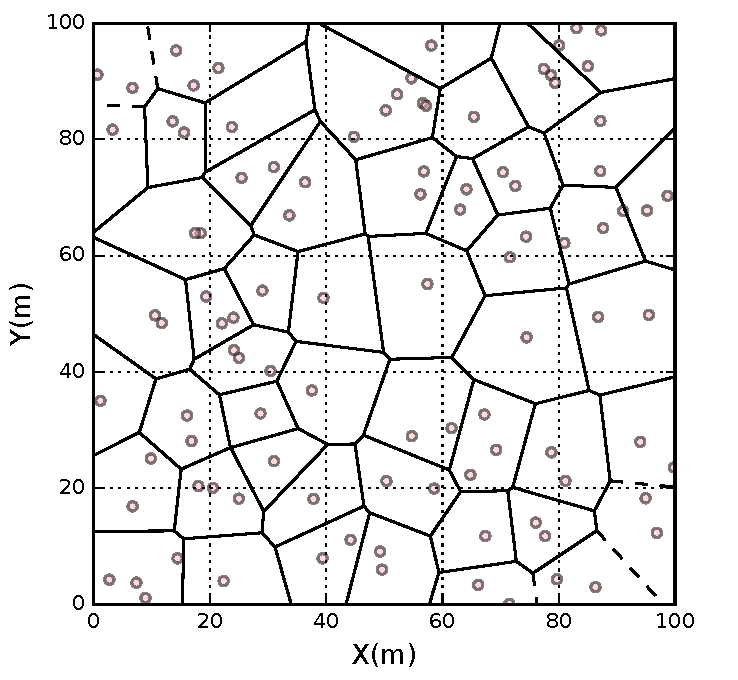
\includegraphics[width = 0.5\textwidth]{kmeans_network_show.pdf}
\caption{基于~k~-~均值的分簇算法的效果图}\vspace{-0.5em}
\label{kmeans_network_show}
\end{figure}
可以看到整个区域被泰森多边形分割,归属于同一个泰森多边形的基站作为一簇,簇内的微基站采用多用户联合传输算法,
多边形内粉色的点表示联合起来的基站。可以看到基站均匀的被分割成了以均值为中心的区域。每个簇内大约有~5~个微基站。

对以用户为中心的基站分簇算法进行仿真,

\BiSubsection{性能优化算法的性能分析}{cluster}
基于前两节的阐述和分析,这一节对密集热点区域无线网络优化后的系统性能与优化之前进行对比,
应用~Python3.5~进行仿真分析,分别仿真了基于深度优先搜索和基于~k~-~均值的基站分簇算法对基站进行分簇,
采用基于~ZFBF~的多用户联合传输干扰消除技术对网络进行优化,以覆盖率作为目标参数对系统的性能进行分析。
具体的仿真参数如表~\ref{cluster_zfbf_sim_para}~所示。
\begin{table}[htbp]
\caption{密集热点区域无线网络的性能优化的仿真参数设定}
\label{cluster_zfbf_sim_para}
\vspace{0.5em}\centering\wuhao
\begin{tabular}{cccc}
\toprule[1.5pt]
参量 & & & 设置 \\
\midrule[0.5pt]
基站的分布~$\Phi$~ & & & 泊松点过程 \\
用户的分布~$\Psi$~  & & & 混合二维高斯分布\\
用户的分散程度~$\sigma$~ & & &  ~$5\mathrm{m}$~ \\
区域~$\mathcal{D}$~的大小  & & & ~$100\mathrm{m} \times 100 \mathrm{m}$~ \\
微基站的天线数 & & & 1 \\
基站的最大发射功率~$P$~ & & & 1 \\
用户的天线数 & & & 1 \\
服务基站的选择方式 & & & 簇内多用户联合传输 \\
门限参数~$\tau$~ & & & ~$3\mathrm{m}$,~$5\mathrm{m}$,~$7\mathrm{m}$~ \\
均值个数~$k$~ & & & ~$30,~50,~70$~ \\
$\mathrm{SINR}$ & & & $-10 \sim 20$~dB \\
\bottomrule[1.5pt]
\end{tabular}
\end{table}

本章基于第~3~章提出并分析的网络模型进行优化,基站的分布为泊松点过程,用户的分布为混合二维高斯分布,
不失一般性,选取用户的分散程度~$\sigma = 5 \mathrm{m}$,
区域~$\mathcal{D}$~的大小为~$100\mathrm{m} \times 100 \mathrm{m}$,基站和用户的天线数均为~1~个,
基站的发射功率为~1,链路为下行链路,考虑的基站分簇方案分别为基于深度优先搜索和基于~k~-~均值的基站分簇策略。
簇内采用多用户联合传输,簇内随机选择用户进行服务。
对于基于深度优先搜索的微基站分簇算法,考虑门限参数为~$3\mathrm{m}$,$5\mathrm{m}$,$7\mathrm{m}$~的情况。
对于基于~k~-~均值的微基站分簇算法,考虑门限均值个数为~5,~10,~15~个的情况。

应用基于深度优先搜索的微基站分簇算法进行分簇,
采用基于~ZFBF~的簇内多用户多基站联合传输的干扰消除技术对网络的性能进行优化,
得到的性能结果仿真曲线如图~\ref{dfs_zfbf_sim_show}~所示:
\begin{figure}[htbp]
\centering
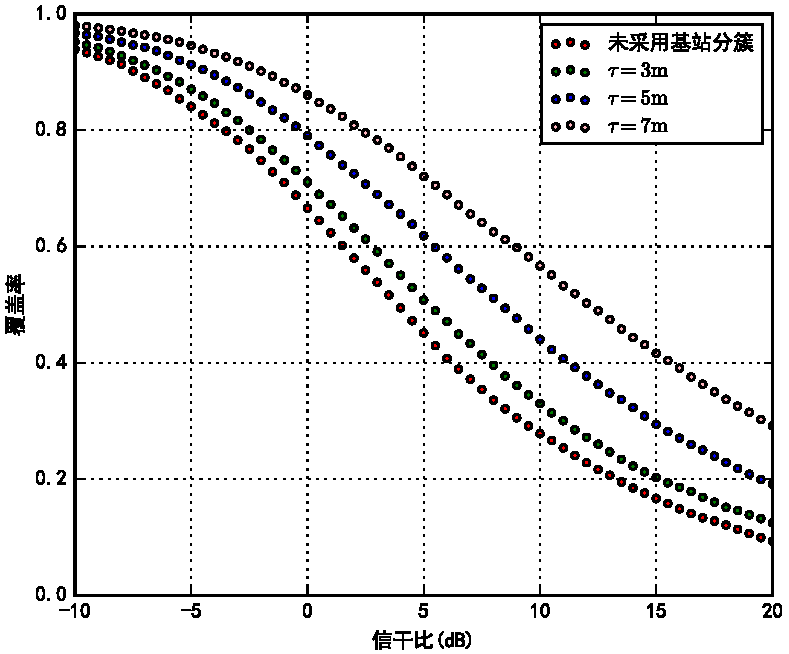
\includegraphics[width = 0.62\textwidth]{dfs_zfbf_sim_show.pdf}
\caption{基于深度优先搜索的基站分簇与多用户联合传输算法性能仿真图}\vspace{-0.5em}
\label{dfs_zfbf_sim_show}
\end{figure}
图~\ref{dfs_zfbf_sim_show}~对基于深度优先搜索的基站分簇算法的分簇策略
并基于~ZFBF~干扰消除技术进行簇内多用户联合传输这种干扰管理策略进行了仿真分析,
并与未采用基站分簇时的情况进行了比较。设定距离门限~$\tau=3\mathrm{m}$,~$5\mathrm{m}$,~$7\mathrm{m}$。

根据仿真结果可以看出,基于深度优先搜索的基站分簇算法和基于联合传输的干扰管理策略有效的提高了小区的覆盖率性能。
其中,随着距离门限~$\tau$~的提升,系统的覆盖率的性能越来越好,
但随着距离门限~$\tau$~的提升,联合的基站的个数也是逐渐提高。
系统的复杂度也逐渐提升,对~CRAN~架构的前向回程链路的容量需求也就越大。
在实际的网络中,可以根据性能和复杂度的折中合理的选择距离门限~$\tau$~这个超参数。

应用基于~k~-~均值的微基站分簇算法进行分簇,
采用基于~ZFBF~的簇内多用户多基站联合传输的干扰消除技术对网络的性能进行优化,
得到的性能结果仿真曲线如图~\ref{kmeans_zfbf_sim_show}~所示:
\begin{figure}[htbp]
\centering
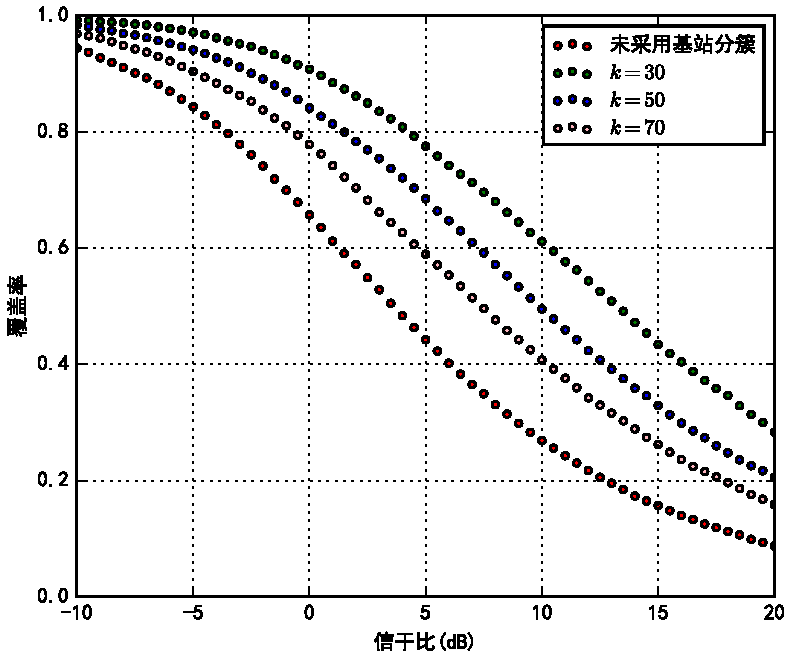
\includegraphics[width = 0.62\textwidth]{kmeans_zfbf_sim_show.pdf}
\caption{基于~k~-~均值的基站分簇与多用户联合传输算法性能仿真图}\vspace{-0.5em}
\label{kmeans_zfbf_sim_show}
\end{figure}

图~\ref{dfs_zfbf_sim_show}~对基于~k~-~均值的基站分簇算法的分簇策略
并基于~ZFBF~干扰消除技术进行簇内多用户联合传输这种干扰管理策略进行了仿真分析,
并与未采用基站分簇时的情况进行了比较,设定的均值个数分别为~$30,~50,~70$~ 个。

根据仿真结果可以看出,基于~k~-~均值的基站分簇算法进行分簇
并基于联合传输进行干扰管理有效的提高了小区的覆盖率性能。
其中,随着均值个数降低,簇的密度降低,簇内联合的基站的个数提高,系统的覆盖率的性能越来越好,
但随簇的个数降低离,联合的基站的个数也是逐渐提高,复杂度逐渐提升,系统对计算能力的需求逐渐提高,
对~CRAN~系统的前向链路的容量需求也逐渐提高。

根据第三章得到的结果,网络的单位面积谱效率是对网络的覆盖率求积分的形式,因此,网络的单位面积谱效率
和网络的中断概率是正相关的,提升了网络的覆盖率,也说明网络的单位面积谱效率也得到了提升。

\BiSection{本章小结}{Conclusion}

本章主要对密集热点区域无线网络的网络性能进行了优化,
首先,提出了两种小区内微基站的分簇算法,分别为基于深度优先搜索的微基站分簇算法,
和基于~k~-~均值的微基站分簇算法。
接着提出了多用户联合传输算法用于基站内的干扰管理,其中网络架构采用基于~CRAN~的网络架构,
簇内基站联合采用分布式~ZFBF~技术。

经过仿真实验证明,
基于首先对基站进行分簇,再对簇内进行干扰消除的干扰管理算法有效的提高了网络的覆盖率性能,
从而也说明有效的提高了网络的单位面积谱效率。
